%% Draft of probabilistic interpretation of quantization
\section{Probabilistic Interpretation of Quantization}
\begin{frame}{Probability distribution of the output of a quantizer}
\textbf{Question:} what's the probability density function (PDF) $p_{x_Q}(x)$ of the quantizer output $x_Q[n] \sim p_{x_Q}(x)$ when the input signal $x[n]$ has PDF $x[n] \sim p_{x}(x)$?
\begin{center}
	\resizebox{0.75\textwidth}{!}{\begin{tikzpicture}
\begin{axis}[
name=plot1,
width=\textwidth,
height=0.5\textwidth,
axis lines*=middle,
enlargelimits = upper, clip=true,
scale only axis,
axis line style={->,>=stealth},
xlabel={\Large $x$},
ylabel={\Large $p_x(x)$},
every axis x label/.style={
	at={(ticklabel* cs:1)},
	xshift=-0.2cm,
	anchor=north,
},
every axis y label/.style={
	at={(ticklabel* cs:0.9)},
	xshift=0.7cm,
	anchor=south,
},
every outer x axis line/.append style={white!15!black},
every x tick label/.append style={font=\color{white!15!black}},
xmin=-3.00, xmax=3.4,
ymin=0, ymax=0.5,
ytick=\empty,
xtick={-2.5, -1.5, -0.5, 0.5, 1.5, 2.5},
xticklabels={\large $-\frac{5\Delta}{2}$, \large$-\frac{3\Delta}{2}$, \large$-\frac{\Delta}{2}$,\large $\frac{\Delta}{2}$, \large$\frac{3\Delta}{2}$, \large$\frac{5\Delta}{2}$},
xmajorgrids,
ymajorgrids,
every outer y axis line/.append style={white!15!black},
every y tick label/.append style={font=\color{white!15!black}},
legend style={draw=white!15!black,fill=white,legend cell align=left, at={(axis cs: 3, 0.25)}}]

\addplot [name path=g, smooth, black, line width=1.5pt, domain=-5:5, samples=51, forget plot] {gauss(x)};
\path[name path=axis1] (axis cs:-0.5,0) -- (axis cs:0.5,0);

\addplot [
thick,
color=black,
fill=black, 
fill opacity=0.10,
forget plot,
]
fill between[
of=g and axis1,
soft clip={domain=-0.5:0.5},
];

\node[black, fill=black!10, minimum size=1cm] at (axis cs: 1.75, 0.45) {\Large $\mathrm{Pr}(-\Delta/2 \leq x \leq \Delta/2)$};

\only<3-|handout:1>{
\addplot [dirac, line width=1.5pt] coordinates {(-2, 0.05) (-1, 0.15) (0, 0.3) (1, 0.15) (2, 0.05)}; \addlegendentry{\Large $p_{x_Q}(x)$};
}

\only<2-|handout:1>{
	\addplot [dirac, line width=1.5pt, forget plot] coordinates {(0, 0.3)};
}
\end{axis}
\end{tikzpicture}
}
\end{center}

\onslide<4|handout:1>{
The PDF of $x_Q[n] \sim p_{x_Q}(x)$ is formed by impulses at the quantization levels. The area of any given impulse is equal to the area under $p_x(x)$ in the quantization interval corresponding to that impulse. In the example of the figure, the area of the impulse at the origin is equal to the highlighted area under $p_x(x)$.
}
\end{frame}

%
\begin{frame}{Area sampling}
We can view $p_{x_Q}(x)$ as samples of the area of $p_x(x)$ under quantization intervals. This form of sampling is called \textbf{area sampling}.

\begin{equation*}
p_{x_Q}(x) = \underbrace{(p_x(x) \ast r(x))}_{\text{\normalsize area calculation}}\overbrace{\cdot s(x)}^{\text{\normalsize sampling}},
\end{equation*}
where 
\begin{equation*}
r(x) = \begin{cases}
\frac{1}{\Delta}, & -\frac{\Delta}{2} \leq x \leq \frac{\Delta}{2} \\
0, & \text{otherwise}
\end{cases} \tag{rectangular window of area 1}
\end{equation*}

\begin{equation*}
s(x) = \sum_{n = -\infty}^{\infty} \delta(x - n\Delta) \tag{impulse train}
\end{equation*}
The period of the impulse train (\textit{sampling period}) is $\Delta$

\textbf{Interesting:} although quantization is an nonlinear operation on the signal, it is a linear operation on that signal PDF, since area sampling is linear.
\end{frame}

%
\begin{frame}{Area sampling: graphically}
\begin{center}
	\resizebox{0.9\textwidth}{!}{\begin{tikzpicture}
\onslide<1-|handout:1>{
\begin{axis}[
	name=plot1,
	axis lines*=middle,
	enlargelimits = upper, clip=true,
	scale only axis,
	width=\textwidth,
	height=0.2\textwidth,
	ymin=0, ymax=0.5,
	xmin=-5, xmax=5,
	axis line style={->,>=stealth},
	xlabel={\small $x$},
	ylabel={\small $p_x(x)$},
	every axis x label/.style={
		at={(ticklabel* cs:1)},
		anchor=north,
	},
	every axis y label/.style={
		at={(ticklabel* cs:0.8)},
		anchor=south,
		xshift=0.6cm,
	},
	xtick={-3,...,3},
	xticklabels={$-3\Delta$,$-2\Delta$, $-\Delta$, 0, $\Delta$, $2\Delta$, $3\Delta$},
	ytick=\empty,
	every outer y axis line/.append style={white!15!black},
	every y tick label/.append style={font=\color{white!15!black}},
	legend style={draw=white!15!black,fill=white,legend cell align=left}]
	\addplot[smooth, line width=1pt, domain=-5:5, samples=31] {gauss(x)};
\end{axis}
}

\onslide<2-|handout:1>{
\begin{axis}[
	name=plot2,
	at=(plot1.below south east), anchor=above north east,
	axis lines*=middle,
	enlargelimits = upper, clip=true,
	scale only axis,
	width=\textwidth,
	height=0.2\textwidth,
	ymin=0, ymax=1.5,
	xmin=-5, xmax=5,
	axis line style={->,>=stealth},
	xlabel={\small $x$},
	ylabel={\small $r(x)$},
	every axis x label/.style={
		at={(ticklabel* cs:1)},
		anchor=north,
	},
	every axis y label/.style={
		at={(ticklabel* cs:0.8)},
		anchor=south,
		xshift=0.6cm,
	},
	xtick={-0.5, 0.5},
	ytick=1,
	yticklabels={$\frac{1}{\Delta}$},
	yticklabel style={yshift=0.3cm},
	xticklabels={$-\frac{\Delta}{2}$, $\frac{\Delta}{2}$}, 
	every outer y axis line/.append style={white!15!black},
	every y tick label/.append style={font=\color{white!15!black}},
	legend style={draw=white!15!black,fill=white,legend cell align=left}]
	\addplot[solid, line width=1pt] coordinates {(-5, 0) (-1/2, 0) (-1/2, 1) (1/2, 1) (1/2, 0) (5, 0)};
\end{axis}
}

\onslide<3|handout:0>{
	\begin{axis}[
	name=plot3,
	at=(plot2.below south east), anchor=above north east,
	axis lines*=middle,
	enlargelimits = upper, clip=true,
	scale only axis,
	width=\textwidth,
	height=0.2\textwidth,
	ymin=0, ymax=0.5,
	xmin=-5, xmax=5,
	axis line style={->,>=stealth},
	xlabel={\small $x$},
	ylabel={\small $p_x(x) \ast r(x)$},
	every axis x label/.style={
		at={(ticklabel* cs:1)},
		anchor=north,
	},
	every axis y label/.style={
		at={(ticklabel* cs:0.8)},
		anchor=south,
		xshift=1cm,
	},
	xtick=\empty,
	ytick=\empty,
	every outer y axis line/.append style={white!15!black},
	every y tick label/.append style={font=\color{white!15!black}},
	legend style={draw=white!15!black,fill=white,legend cell align=left}]
\addplot [smooth, line width=1pt, forget plot]
table[row sep=crcr]{
	-5 3.1178e-06 \\
-4.8 8.1063e-06 \\
-4.6 1.9895e-05 \\
-4.4 4.6364e-05 \\
-4.2 0.00010396 \\
-4 0.00022431 \\
-3.8 0.00046577 \\
-3.6 0.0009308 \\
-3.4 0.0017904 \\
-3.2 0.0033151 \\
-3 0.0059093 \\
-2.8 0.010142 \\
-2.6 0.01676 \\
-2.4 0.026672 \\
-2.2 0.040879 \\
-2 0.060346 \\
-1.8 0.085813 \\
-1.6 0.11756 \\
-1.4 0.15515 \\
-1.2 0.1973 \\
-1 0.24176 \\
-0.8 0.28547 \\
-0.6 0.32484 \\
-0.4 0.35623 \\
-0.2 0.3765 \\
0 0.38351 \\
0.2 0.3765 \\
0.4 0.35623 \\
0.6 0.32484 \\
0.8 0.28547 \\
1 0.24176 \\
1.2 0.1973 \\
1.4 0.15515 \\
1.6 0.11756 \\
1.8 0.085813 \\
2 0.060346 \\
2.2 0.040879 \\
2.4 0.026672 \\
2.6 0.01676 \\
2.8 0.010142 \\
3 0.0059093 \\
3.2 0.0033151 \\
3.4 0.0017904 \\
3.6 0.0009308 \\
3.8 0.00046577 \\
4 0.00022431 \\
4.2 0.00010396 \\
4.4 4.6364e-05 \\
4.6 1.9895e-05 \\
4.8 8.1063e-06 \\
5 3.1178e-06 \\
};

\end{axis}
}


\onslide<4-|handout:1>{
	\begin{axis}[
	name=plot3,
	at=(plot2.below south east), anchor=above north east,
	axis lines*=middle,
	enlargelimits = upper, clip=true,
	scale only axis,
	width=\textwidth,
	height=0.2\textwidth,
	ymin=0, ymax=0.5,
	xmin=-5, xmax=5,
	axis line style={->,>=stealth},
	xlabel={\small $x$},
	ylabel={\small $p_{x_Q}(x) = (p_x(x) \ast r(x))\cdot s(x)$},
	every axis x label/.style={
		at={(ticklabel* cs:1)},
		anchor=north,
	},
	every axis y label/.style={
		at={(ticklabel* cs:0.8)},
		anchor=south,
		xshift=2.3cm,
	},
	xtick={-3,...,3},
	xticklabels={$-3\Delta$,$-2\Delta$, $-\Delta$, 0, $\Delta$, $2\Delta$, $3\Delta$},
	ytick=\empty,
	every outer y axis line/.append style={white!15!black},
	every y tick label/.append style={font=\color{white!15!black}},
	legend style={draw=white!15!black,fill=white,legend cell align=left}]
	\addplot [smooth, black!20, line width=1pt, forget plot]
	table[row sep=crcr]{
		-5 3.1178e-06 \\
		-4.8 8.1063e-06 \\
		-4.6 1.9895e-05 \\
		-4.4 4.6364e-05 \\
		-4.2 0.00010396 \\
		-4 0.00022431 \\
		-3.8 0.00046577 \\
		-3.6 0.0009308 \\
		-3.4 0.0017904 \\
		-3.2 0.0033151 \\
		-3 0.0059093 \\
		-2.8 0.010142 \\
		-2.6 0.01676 \\
		-2.4 0.026672 \\
		-2.2 0.040879 \\
		-2 0.060346 \\
		-1.8 0.085813 \\
		-1.6 0.11756 \\
		-1.4 0.15515 \\
		-1.2 0.1973 \\
		-1 0.24176 \\
		-0.8 0.28547 \\
		-0.6 0.32484 \\
		-0.4 0.35623 \\
		-0.2 0.3765 \\
		0 0.38351 \\
		0.2 0.3765 \\
		0.4 0.35623 \\
		0.6 0.32484 \\
		0.8 0.28547 \\
		1 0.24176 \\
		1.2 0.1973 \\
		1.4 0.15515 \\
		1.6 0.11756 \\
		1.8 0.085813 \\
		2 0.060346 \\
		2.2 0.040879 \\
		2.4 0.026672 \\
		2.6 0.01676 \\
		2.8 0.010142 \\
		3 0.0059093 \\
		3.2 0.0033151 \\
		3.4 0.0017904 \\
		3.6 0.0009308 \\
		3.8 0.00046577 \\
		4 0.00022431 \\
		4.2 0.00010396 \\
		4.4 4.6364e-05 \\
		4.6 1.9895e-05 \\
		4.8 8.1063e-06 \\
		5 3.1178e-06 \\
	};
	
	\addplot [dirac, line width=1pt, forget plot]
	table[row sep=crcr]{
		-2 0.053991 \\
		-1 0.24197 \\
		0 0.39894 \\
		1 0.24197 \\
		2 0.053991 \\
	};
	\end{axis}
}

\end{tikzpicture}
}
\end{center}	
\end{frame}

%
\begin{frame}{Random variables and convolution}
The area sampling interpretation of quantization gives us a simple equation for the PDF of $x_Q[n]$:
\begin{equation*}
p_{x_Q}(x) = \underbrace{(p_x(x) \ast r(x))}_{\text{\normalsize area calculation}}\overbrace{\cdot s(x)}^{\text{\normalsize sampling}},
\end{equation*}

\pause
\textbf{Another interpretation:} in probability theory, we use convolution to calculate the PDF of the \textbf{sum of two independent random variables}:

\begin{equation*}
Z = X + Y \Longrightarrow p_Z = p_X \ast p_Y
\end{equation*}

\pause
Applying to our problem:

\begin{equation*}
\tilde{x}_Q[n] = x[n] + q[n] \Longrightarrow p_{\tilde{x}_Q}(x) = \underbrace{(p_x(x) \ast r(x))}_{\text{\normalsize area calculation}}
\end{equation*}
where $q[n]$ is a random variable independent of $x[n]$ and with PDF $p_q(x) = r(x)$. Therefore, $q$ is an \textbf{uniform random variable} ($q\sim\mathcal{U}[-\Delta/2, \Delta/2]$).
\end{frame}

%
\begin{frame}
Comparing with the definition of quantization error:
\begin{align*}
x_Q[n] &= x[n] - e[n] \tag{from definition of quantization error} \\
\tilde{x}_Q[n] &= x[n] + q[n] \tag{from probabilistic interpreation of area sampling}
\end{align*}

The equations for $x_Q[n]$ and $\tilde{x}_Q[n]$ are very similar, but there's an important difference. The PDF $p_{x_Q}(x)$ is formed by \textbf{sampling} $p_{\tilde{x}_Q}(x)$.

\pause
\begin{center}
	\resizebox{0.55\textwidth}{!}{\begin{tikzpicture}
\begin{axis}[
	axis lines*=middle,
	enlargelimits = upper, clip=true,
	scale only axis,
	width=0.8\textwidth,
	height=0.4\textwidth,
	ymin=0, ymax=0.4,
	xmin=-4, xmax=4,
	axis line style={->,>=stealth},
	xlabel={\Large $x$},
	ylabel={\huge $p_{x_Q}(x) = \underbrace{(p_x(x) \ast r(x))}_{\Large p_{\tilde{x}_Q}(x)}\cdot s(x)$},
	every axis x label/.style={
		at={(ticklabel* cs:1)},
		anchor=north,
	},
	every axis y label/.style={
		at={(ticklabel* cs:0.8)},
		anchor=south,
		xshift=2.3cm,
	},
	xtick={-3,...,3},
	xticklabels={$-3\Delta$,$-2\Delta$, $-\Delta$, 0, $\Delta$, $2\Delta$, $3\Delta$},
	ytick=\empty,
	every outer y axis line/.append style={white!15!black},
	every y tick label/.append style={font=\color{white!15!black}},
	legend style={draw=white!15!black,fill=white,legend cell align=left}]
	\addplot [smooth, black!20, line width=1pt, forget plot]
	table[row sep=crcr]{
		-5 3.1178e-06 \\
		-4.8 8.1063e-06 \\
		-4.6 1.9895e-05 \\
		-4.4 4.6364e-05 \\
		-4.2 0.00010396 \\
		-4 0.00022431 \\
		-3.8 0.00046577 \\
		-3.6 0.0009308 \\
		-3.4 0.0017904 \\
		-3.2 0.0033151 \\
		-3 0.0059093 \\
		-2.8 0.010142 \\
		-2.6 0.01676 \\
		-2.4 0.026672 \\
		-2.2 0.040879 \\
		-2 0.060346 \\
		-1.8 0.085813 \\
		-1.6 0.11756 \\
		-1.4 0.15515 \\
		-1.2 0.1973 \\
		-1 0.24176 \\
		-0.8 0.28547 \\
		-0.6 0.32484 \\
		-0.4 0.35623 \\
		-0.2 0.3765 \\
		0 0.38351 \\
		0.2 0.3765 \\
		0.4 0.35623 \\
		0.6 0.32484 \\
		0.8 0.28547 \\
		1 0.24176 \\
		1.2 0.1973 \\
		1.4 0.15515 \\
		1.6 0.11756 \\
		1.8 0.085813 \\
		2 0.060346 \\
		2.2 0.040879 \\
		2.4 0.026672 \\
		2.6 0.01676 \\
		2.8 0.010142 \\
		3 0.0059093 \\
		3.2 0.0033151 \\
		3.4 0.0017904 \\
		3.6 0.0009308 \\
		3.8 0.00046577 \\
		4 0.00022431 \\
		4.2 0.00010396 \\
		4.4 4.6364e-05 \\
		4.6 1.9895e-05 \\
		4.8 8.1063e-06 \\
		5 3.1178e-06 \\
	} node[pos=0.65, black, pin={[pin edge={black, thick}]40:{\color{black} \Large $p_{\tilde{x}_Q}(x)$}}, inner sep=0pt] {};

	
	\addplot [dirac, line width=1pt, forget plot]
	table[row sep=crcr]{
		-2 0.053991 \\
		-1 0.24197 \\
		0 0.39894 \\
		1 0.24197 \\
		2 0.053991 \\
	};
\end{axis}
\end{tikzpicture}}
\end{center}

\pause
If the sampled PDF ($p_{x_Q}(x)$) perfectly describes $p_{\tilde{x}_Q}(x)$, we can say that quantization error is perfectly described by an uniform random process.

\pause 
\textbf{Question:}  under what conditions can we perfectly reconstruct $p_{\tilde{x}_Q}(x)$ from its samples? \\
\end{frame}

%
\begin{frame}{Revisiting the Shannon-Nyquist theorem}
	Recall that the \textbf{Shannon-Nyquist theorem} guarantees that we can perfectly recover a signal from its samples if two conditions are met:
	\begin{enumerate}
		\item \textbf{No aliasing; spectrum replicas do not overlap}
		\item Use ideal reconstruction filter (ideal lowpass filter)
	\end{enumerate}
	\pause
	\begin{block}{Conditions for no aliasing}
		\begin{enumerate}
			\item The \textbf{characteristic function} (Fourier transform) of the area-sampled input PDF must satisfy: 
			\begin{equation*}
				\Phi_{p_{x_Q}}(j\theta) = \mathcal{F}\{p_{x_Q}(x)\} = 0, |\theta| > \theta_N
			\end{equation*}
			This is analogous to the condition of a signal being \textit{band-limited}.
			\item\pause The \textit{sampling frequency} $\theta_s$ must be such that $\theta_s > 2\theta_N$.
			
			In this context, $\theta_s = 2\pi/\Delta$, and the quantization interval $\Delta$ is equivalent to the \textit{sampling period} (period of the impulse train).
		\end{enumerate}
	\end{block}
\end{frame}

%
\begin{frame}<beamer:0|handout:1>
Additional comments
\begin{itemize}
	\item When we used the Shannon-Nyquist theorem for sampling a continuous-time signal, we said that we can use an anti-aliasing filter to minimize aliasing, but we could not use the ideal lowpass filter, as it is unfeasible.
	\item In this discussion on quantization, we just want theoretical assurance that we can reconstruct the PDF from its samples. Therefore, for this purpose, we can use the ideal lowpass filter.
	\item On the other hand, we cannot guarantee that there won't be aliasing, as many probability distributions are not \textit{band-limited}.
\end{itemize}
\end{frame}

%
\begin{frame}
	\textbf{Conclusion:} if the conditions for no aliasing are met, we can perfectly reconstruct the original PDF from its samples, and therefore, quantization noise can be \underline{perfectly modeled} as an uniform random process.
	
	\pause
	\textbf{Bad news:} the conditions for no aliasing are generally not met in practice. \textbf{Example:} Gaussian distribution. The characteristic function of the Gaussian distribution is a Gaussian function. The Gaussian function is not \textit{band-limited}, as it is always non-zero.
	
	\pause
	\textbf{How can we mitigate aliasing?}
	\begin{enumerate}
		\item Anti-aliasing filter? This would be equivalent to modify the PDF of the input signal. But what would it do the signal?
		\item Oversampling $\implies$ shorter sampling period ($\Delta$) $\implies$ finer quantization
	\end{enumerate}
\end{frame}

% 
\begin{frame}{Example for the Gaussian input distribution}
	\begin{itemize}
		\item A zero-mean Gaussian distributed signal with variance $\sigma^2$ is quantized with quantization resolution \tikz[baseline]{\node[fill=black!10,anchor=base] {$\Delta = 2.1\sigma$};}
		\item Overlap of spectrum replicas results in \underline{significant aliasing}
		\item The estimated quantization noise PDF differs from the uniform distribution
	\end{itemize}
	
	\begin{columns}[t]
		\begin{column}{0.5\textwidth}
			Fourier transform of sampled PDF
				\begin{center}
					\resizebox{\textwidth}{!}{\PlotGaussianCF{figs/aliased_gaussian_cf.tex}{1}{2.9920}{$\Delta = 2.1\sigma$}}
				\end{center}
		\end{column}
			\begin{column}{0.5\textwidth}
			Estimated quantization noise PDF
			\begin{center}
					\resizebox{0.9\textwidth}{!}{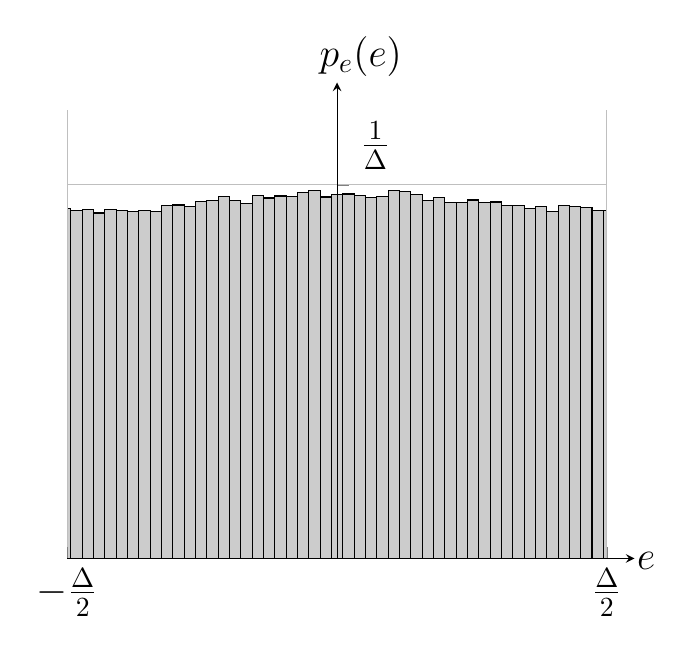
\begin{tikzpicture}
\begin{axis}[
xmin=-1, xmax=1,
axis lines*=center,
every axis y label/.style={at=(current axis.above origin),anchor=south},
every axis x label/.style={at=(current axis.right of origin),anchor=west},
%height=5cm, width=8cm,
xtick=\empty,
ytick=\empty,
xticklabel=\empty,
ymin=0,
ymax=0.6,
yticklabel style={yshift=0.5cm, xshift=0.8cm},
ylabel={\Large $p_{e}(e)$},
xlabel={\Large $e$},
enlargelimits=false, clip=true, axis on top,
grid = major,
axis line style={->,>=stealth, shorten >= -10pt},
every axis x label/.style={
	at={(ticklabel* cs:1)},
	yshift=0.2cm,
	xshift=0.5cm,
	anchor=north,
},
every axis y label/.style={
	at={(ticklabel* cs:1)},
	anchor=south,
	xshift=0.3cm,
	yshift=0.3cm,
},
xtick={-1, 1},
ytick=0.5,
yticklabels={\Large $\frac{1}{\Delta}$},
xticklabels={\Large$-\frac{\Delta}{2}$, \Large $\frac{\Delta}{2}$},
]
\addplot[black, ybar interval, fill=black!20, mark=no] 
table[row sep=crcr]{
	-1.029 0.4681 \\
	-0.987 0.46555 \\
	-0.945 0.46698 \\
	-0.903 0.46238 \\
	-0.861 0.46662 \\
	-0.819 0.46579 \\
	-0.777 0.46467 \\
	-0.735 0.46533 \\
	-0.693 0.4645 \\
	-0.651 0.47183 \\
	-0.609 0.473 \\
	-0.567 0.47052 \\
	-0.525 0.47769 \\
	-0.483 0.47964 \\
	-0.441 0.4845 \\
	-0.399 0.47945 \\
	-0.357 0.4756 \\
	-0.315 0.48581 \\
	-0.273 0.48245 \\
	-0.231 0.48512 \\
	-0.189 0.48455 \\
	-0.147 0.48971 \\
	-0.105 0.49229 \\
	-0.062999 0.48376 \\
	-0.020999 0.48714 \\
	0.021001 0.48774 \\
	0.063 0.48517 \\
	0.105 0.48286 \\
	0.147 0.48495 \\
	0.189 0.49255 \\
	0.231 0.49062 \\
	0.273 0.48731 \\
	0.315 0.47883 \\
	0.357 0.48307 \\
	0.399 0.4764 \\
	0.441 0.47657 \\
	0.483 0.47974 \\
	0.525 0.47679 \\
	0.567 0.47707 \\
	0.609 0.47186 \\
	0.651 0.47183 \\
	0.693 0.46886 \\
	0.735 0.4711 \\
	0.777 0.46469 \\
	0.819 0.47233 \\
	0.861 0.47057 \\
	0.903 0.46924 \\
	0.945 0.46526 \\
	0.987 0.46519 \\
	1.029 0.46595 \\
};
\addplot[black, domain=-1:1, samples=2] {0.5};
\end{axis}
\end{tikzpicture}}
			\end{center}
			\end{column}
	\end{columns}
\end{frame}

%
\begin{frame}{Example for the Gaussian input distribution}
\begin{itemize}
	\item A zero-mean Gaussian distributed signal with variance $\sigma^2$ is quantized with quantization resolution \tikz[baseline]{\node[fill=black!10,anchor=base] {$\Delta = \sigma$};}
	\item Spectrum replicas are sufficiently apart; \underline{aliasing is negligible}
	\item The estimated quantization noise PDF agrees well with the uniform distribution
\end{itemize}

\begin{columns}[t]
	\begin{column}{0.5\textwidth}
		Fourier transform of sampled PDF
		\begin{center}
			\resizebox{\textwidth}{!}{\PlotGaussianCF{figs/aliased_gaussian_cf.tex}{1}{6.2832}{$\Delta = \sigma$}}
		\end{center}
	\end{column}
	\begin{column}{0.5\textwidth}
		Estimated quantization noise PDF
		\begin{center}
			\resizebox{0.9\textwidth}{!}{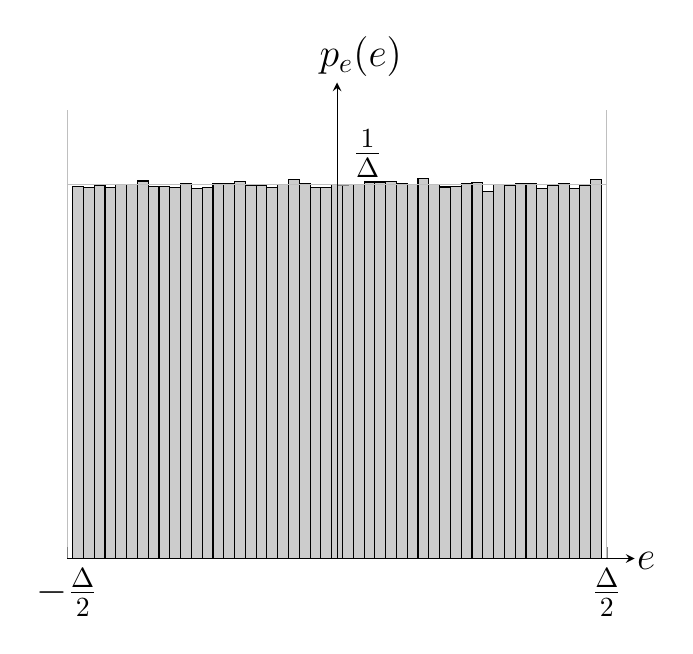
\begin{tikzpicture}
\begin{axis}[
xmin=-0.5,
xmax=0.5,
axis lines*=center,
every axis y label/.style={at=(current axis.above origin),anchor=south},
every axis x label/.style={at=(current axis.right of origin),anchor=west},
%height=5cm, width=8cm,
xtick=\empty,
ytick=\empty,
xticklabel=\empty,
ymin=0,
ymax=1.2,
yticklabel style = {xshift=0.4cm, yshift=-0.2cm},
ylabel={\Large $p_{e}(e)$},
xlabel={\Large  $e$},
enlargelimits=false, clip=true, axis on top,
grid = major,
axis line style={->,>=stealth, shorten >= -10pt},
every axis x label/.style={
	at={(ticklabel* cs:1)},
	yshift=0.2cm,
	xshift=0.5cm,
	anchor=north,
},
every axis y label/.style={
	at={(ticklabel* cs:1)},
	anchor=south,
	xshift=0.3cm,
	yshift=0.3cm,
},
xtick={-0.5, 0.5},
ytick=1,
yticklabel style={yshift=0.6cm, xshift=0.3cm},
yticklabels={\Large $\frac{1}{\Delta}$},
xticklabels={\Large $-\frac{\Delta}{2}$, \Large $\frac{\Delta}{2}$},
]
\addplot[black, ybar interval, fill=black!20, mark=no] 
table[row sep=crcr]{
	-0.49 0.9955 \\
	-0.47 0.992 \\
	-0.45 0.9993 \\
	-0.43 0.99245 \\
	-0.41 1.0013 \\
	-0.39 1.0004 \\
	-0.37 1.0103 \\
	-0.35 0.99475 \\
	-0.33 0.99625 \\
	-0.31 0.99365 \\
	-0.29 1.0048 \\
	-0.27 0.98945 \\
	-0.25 0.9939 \\
	-0.23 1.0035 \\
	-0.21 1.0031 \\
	-0.19 1.0093 \\
	-0.17 0.9976 \\
	-0.15 0.9988 \\
	-0.13 0.99205 \\
	-0.11 1.0021 \\
	-0.09 1.0135 \\
	-0.07 1.0043 \\
	-0.05 0.9941 \\
	-0.03 0.9938 \\
	-0.0099997 1.0017 \\
	0.01 1.0011 \\
	0.03 1.0007 \\
	0.05 1.0078 \\
	0.07 1.0076 \\
	0.09 1.0083 \\
	0.11 1.003 \\
	0.13 1.002 \\
	0.15 1.0163 \\
	0.17 1.0009 \\
	0.19 0.9944 \\
	0.21 0.9965 \\
	0.23 1.0024 \\
	0.25 1.0056 \\
	0.27 0.98185 \\
	0.29 1.0019 \\
	0.31 0.99855 \\
	0.33 1.0045 \\
	0.35 1.0025 \\
	0.37 0.98935 \\
	0.39 0.9994 \\
	0.41 1.0028 \\
	0.43 0.98955 \\
	0.45 0.9975 \\
	0.47 1.0142 \\
	0.49 0.9937 \\
};

\addplot[black, domain=-1:1, samples=2] {1};
\end{axis}
\end{tikzpicture}}
		\end{center}
	\end{column}
\end{columns}
\end{frame}

%
\begin{frame}{Summary on the probabilistic interpretation of quantization}
	\begin{itemize}
		\item In the probability domain, quantization corresponds to area sampling of the input PDF (a linear operation).		
		\item If there's no aliasing (spectrum replicas of area-sampled input PDF do not overlap)
		\begin{enumerate}
			\item Characteristic function of the area-sampled input PDF is \textit{band-limited} with maximum \textit{frequency} $\theta_N$
			\item Sampling period $\Delta$ satisfies $\Delta < \pi/\theta_N$
		\end{enumerate}
		the quantization error is \underline{perfectly modeled} by an uniform random process.
		\item In general aliasing cannot be avoided, but oversampling (finer quantization) makes aliasing negligible and consequently we can still accurately model quantization error as an uniform random process.  
	\end{itemize}
\end{frame}